%%%%%%%%%%%%%%%%%%%%%%%%%%%%%%%%%%%%%%%%%
% Beamer Presentation
% LaTeX Template
% Version 1.0 (10/11/12)
%
% This template has been downloaded from:
% http://www.LaTeXTemplates.com
%
% License:
% CC BY-NC-SA 3.0 (http://creativecommons.org/licenses/by-nc-sa/3.0/)
%
%%%%%%%%%%%%%%%%%%%%%%%%%%%%%%%%%%%%%%%%%

%----------------------------------------------------------------------------------------
%	PACKAGES AND THEMES
%----------------------------------------------------------------------------------------
\documentclass{beamer}

\mode<presentation> {

% The Beamer class comes with a number of default slide themes
% which change the colors and layouts of slides. Below this is a list
% of all the themes, uncomment each in turn to see what they look like.

%\usetheme{default}
%\usetheme{AnnArbor}
%\usetheme{Antibes}
%\usetheme{Bergen}
%\usetheme{Berkeley}
%\usetheme{Berlin}
%\usetheme{Boadilla}
%\usetheme{CambridgeUS}
%\usetheme{Copenhagen}
%\usetheme{Darmstadt}
%\usetheme{Dresden}
%\usetheme{Frankfurt}
%\usetheme{Goettingen}
%\usetheme{Hannover}
%\usetheme{Ilmenau}
%\usetheme{JuanLesPins}
%\usetheme{Luebeck}
\usetheme{Madrid}
%\usetheme{Malmoe}
%\usetheme{Marburg}
%\usetheme{Montpellier}
%\usetheme{PaloAlto}
%\usetheme{Pittsburgh}
%\usetheme{Rochester}
%\usetheme{Singapore}
%\usetheme{Szeged}
%\usetheme{Warsaw}

% As well as themes, the Beamer class has a number of color themes
% for any slide theme. Uncomment each of these in turn to see how it
% changes the colors of your current slide theme.

%\usecolortheme{albatross}
%\usecolortheme{beaver}
%\usecolortheme{beetle}
%\usecolortheme{crane}
%\usecolortheme{dolphin}
%\usecolortheme{dove}
%\usecolortheme{fly}
%\usecolortheme{lily}
%\usecolortheme{orchid}
%\usecolortheme{rose}
%\usecolortheme{seagull}
%\usecolortheme{seahorse}
%\usecolortheme{whale}
%\usecolortheme{wolverine}

%\setbeamertemplate{footline} % To remove the footer line in all slides uncomment this line
%\setbeamertemplate{footline}[page number] % To replace the footer line in all slides with a simple slide count uncomment this line

%\setbeamertemplate{navigation symbols}{} % To remove the navigation symbols from the bottom of all slides uncomment this line
}
%----------------------------------------------------------------------------------------
\usepackage{graphicx} % Allows including images
\usepackage{booktabs} % Allows the use of \toprule, \midrule and \bottomrule in tables
\setbeamerfont{caption}{size=\scriptsize}
\usepackage{hyperref}
%----------------------------------------------------------------------------------------
%	TITLE PAGE
%----------------------------------------------------------------------------------------
\title[]{ROS Basics} % The short title appears at the bottom of every slide, the full title is only on the title page
%----------------------------------------------------------------------------------------
\author{ARRA / AR2A} % Your name
\institute % Your institution as it will appear on the bottom of every slide, may be shorthand to save space
{
\textbf{A}dvancements for \textbf{R}obotics in \textbf{R}escue \textbf{A}pplications
}
\date{\today} % Date, can be changed to a custom date
%----------------------------------------------------------------------------------------
\AtBeginSection{\frame{\sectionpage}}
%----------------------------------------------------------------------------------------
\begin{document}
%----------------------------------------------------------------------------------------
\begin{frame}
\titlepage % Print the title page as the first slide
\end{frame}
%----------------------------------------------------------------------------------------
\begin{frame}
\frametitle{Overview} % Table of contents slide, comment this block out to remove it
\tableofcontents % Throughout your presentation, if you choose to use \section{} and \subsection{} commands, these will automatically be printed on this slide as an overview of your presentation
\end{frame}
%----------------------------------------------------------------------------------------
%	PRESENTATION SLIDES
%----------------------------------------------------------------------------------------
\begin{frame}{ARRA/AR2A}
\begin{large}\textbf{What do we want?}\end{large}
\begin{itemize}
 \item ARRA / AR2A aims to improve the current state of technology of robotics in rescue applications.
\end{itemize}
\begin{large}\textbf{Who are we?}\end{large}
\begin{itemize}
 \item A volunteer non-profit organisation of robotic enthusiasts.
\end{itemize}
\begin{large}\textbf{How can you help?}\end{large}
\begin{itemize}
 \item Check us out at \url{https://github.com/ar2a}
\end{itemize}
 \vspace{1cm}
\begin{large}\textbf{License information}\end{large}
\begin{itemize}
 \item \textbf{CC-BY-SA 4.0} \url{https://creativecommons.org/licenses/by-sa/4.0/}
\end{itemize}
\end{frame}
%----------------------------------------------------------------------------------------
\section{Introduction}
%----------------------------------------------------------------------------------------
\begin{frame}{History}
\begin{itemize}
 \item 2007: Beginnings as project \textbf{switchyard} at the Stanford Artificial Intelligence Laboratory
 \item 2008: Further development by R\&D company Willow Garage  \href{https://www.willowgarage.com/pages/pr2/overview}{\beamergotobutton{PR2}}
 \begin{itemize}
  \item First release: ROS 1.0 (31st December 2012)
 \end{itemize}
 \item 2013: Adoption of the project responsibilty by the \textbf{Open Source Robotics Foundation} (OSRF)
\end{itemize}

\begin{itemize}
 \item \textbf{Versions}: ROS 1.0, Box Turtle, C Turtle, Diamondback, Electric Emys, Fuerte Turtle, Groovy Galapagos, Hydro Medusa, \textbf{Indigo Igloo}, \textbf{Jade Turtle}
 \begin{itemize}
  \item Latest stable version: \textbf{Indigo Igloo}
  \item Latest version: \textbf{Jade Turtle}
 \end{itemize}
\end{itemize}
\end{frame}
%----------------------------------------------------------------------------------------
\begin{frame}{What is ROS?}
\begin{definition}[ROS]
\textit{The Robot Operating System (ROS) is a flexible framework for writing robot software. It is a collection of tools, libraries, and conventions that aim to simplify the task of creating complex and robust robot behavior across a wide variety of robotic platforms.}
\end{definition}
\end{frame}
%----------------------------------------------------------------------------------------
\begin{frame}{Why ROS?}
 \begin{itemize}
 \item $>$ \textbf{3000} 3rd party packages in the ROS repositories provide solutions for various, in every robotic system reoccuring problems
 \item Integration with Gazebo, OpenCV, PointCloudLibrary, MoveIt
 \item Extensive documentation and support by a \textbf{vibrant community}
 \begin{itemize}
  \item $>$ \textbf{5700} users at the ROS Q\&{}A-Page (70\%-Answer-Rate)
  \item $>$ \textbf{22000} ROS-Wiki pages
 \end{itemize}
 \item Permissive \textbf{BSD}-Lizenz
 \end{itemize}
 \begin{figure}[H]
  \centering
  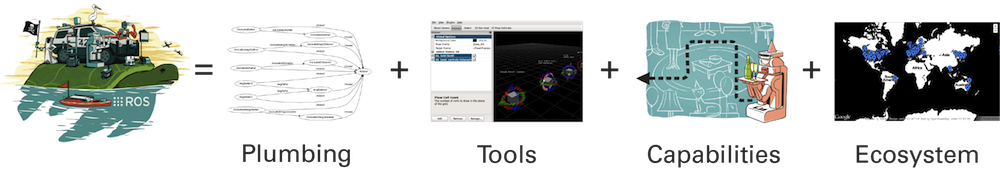
\includegraphics[width=0.85\textwidth]{ros-equation.png}
  \caption{Source: \cite{ROS:2015:Online}}
  \label{fig:ros_equation}
 \end{figure}
\end{frame}
%----------------------------------------------------------------------------------------
\section{Concepts}
%----------------------------------------------------------------------------------------
\begin{frame}{Design Philosophy 1}
 \begin{itemize}
  \item \textbf{Peer-To-Peer}
  \begin{itemize}
   \item Most robotic applications demand a \textbf{huge processing power} 
   \item \textbf{Distributed computing} which performs calculations both on on- and offboard systems required
   \item Interface for data exchange becomes performance bottleneck in systems with a centralised architecture (central server necessary)
  \end{itemize}
 \end{itemize}
 \begin{itemize}
  \item \textbf{Tool based}
  \begin{itemize}
   \item Despite the name \textbf{no operating system but framework} (microkernel approach)
   \item + stability
   \item + expandability
   \item e.g. roscd, roslaunch, rostopic, rosgraph, ...
  \end{itemize}
 \end{itemize}
\end{frame}
%----------------------------------------------------------------------------------------
\begin{frame}{Design Philosophy 2}
 \begin{itemize}
  \item \textbf{Multilingual}
  \begin{itemize}
   \item C++, Python, Octave, Lisp
  \end{itemize}
 \end{itemize}
 \begin{itemize}
  \item \textbf{Thin}
  \begin{itemize}
   \item Wncapsulation of algorithms in libraries
   \begin{itemize}
    \item Communication via defined interfaces
    \item Reusability (algorithms are decoupled from hardware)
    \item Easy to test
   \end{itemize}
  \end{itemize}
 \end{itemize}
 \begin{itemize}
  \item \textbf{Open Source}
  \begin{itemize}
   \item BSD license allows for commercial applications without limitations
  \end{itemize}
 \end{itemize}
\end{frame}
%----------------------------------------------------------------------------------------
\begin{frame}{Node}
\begin{definition}[Node]
\textit{A node is a process performing calculations.}
\end{definition}
 \begin{itemize}
  \item Typical applications consist of multiple nodes
  \item Naming results from graphical representation of all running processes and the communication between thoses processes as \textbf{directed graph} (Tool: \textit{rqt\_graph})
  \item Identifikation of a process by a \textbf{graph ressource name} (''Nodename'')
  \begin{figure}[H]
   \centering
   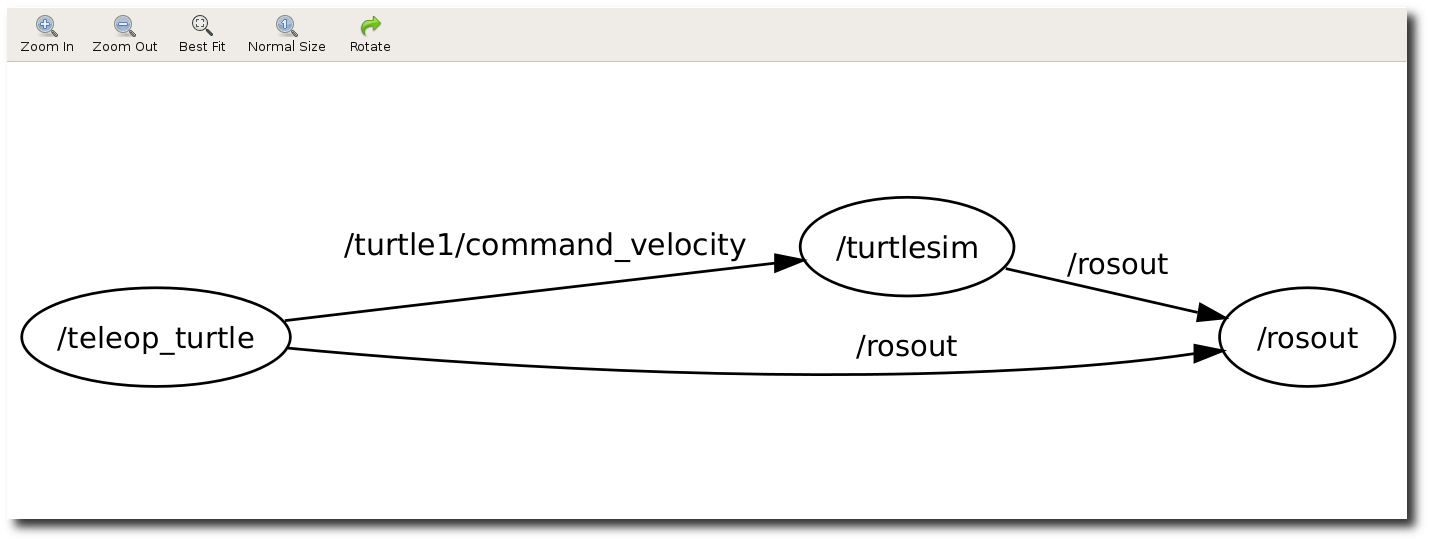
\includegraphics[width=0.6\textwidth]{rxgraph-turtle-key.png}
   \caption{Source: \cite{ROS:2015:Online}}
   \label{fig:ros_graph}
  \end{figure}
 \end{itemize}
\end{frame}
%----------------------------------------------------------------------------------------
\begin{frame}{Topic}
 \begin{definition}[Topic]
 \textit{A topic is a unique name which allows nodes to locate their communication partner for the transmission and reception of data.}
 \end{definition}
 \begin{itemize}
  \item Creation and consumption of data is \textbf{decoupled} (Producer/Consumer-Pattern)
  \begin{itemize}
   \item Source's (\textbf{publish}) data to a topic
   \item Sink's (\textbf{subscribe}) data from a topic
  \end{itemize}
  \begin{figure}[H]
   \centering
   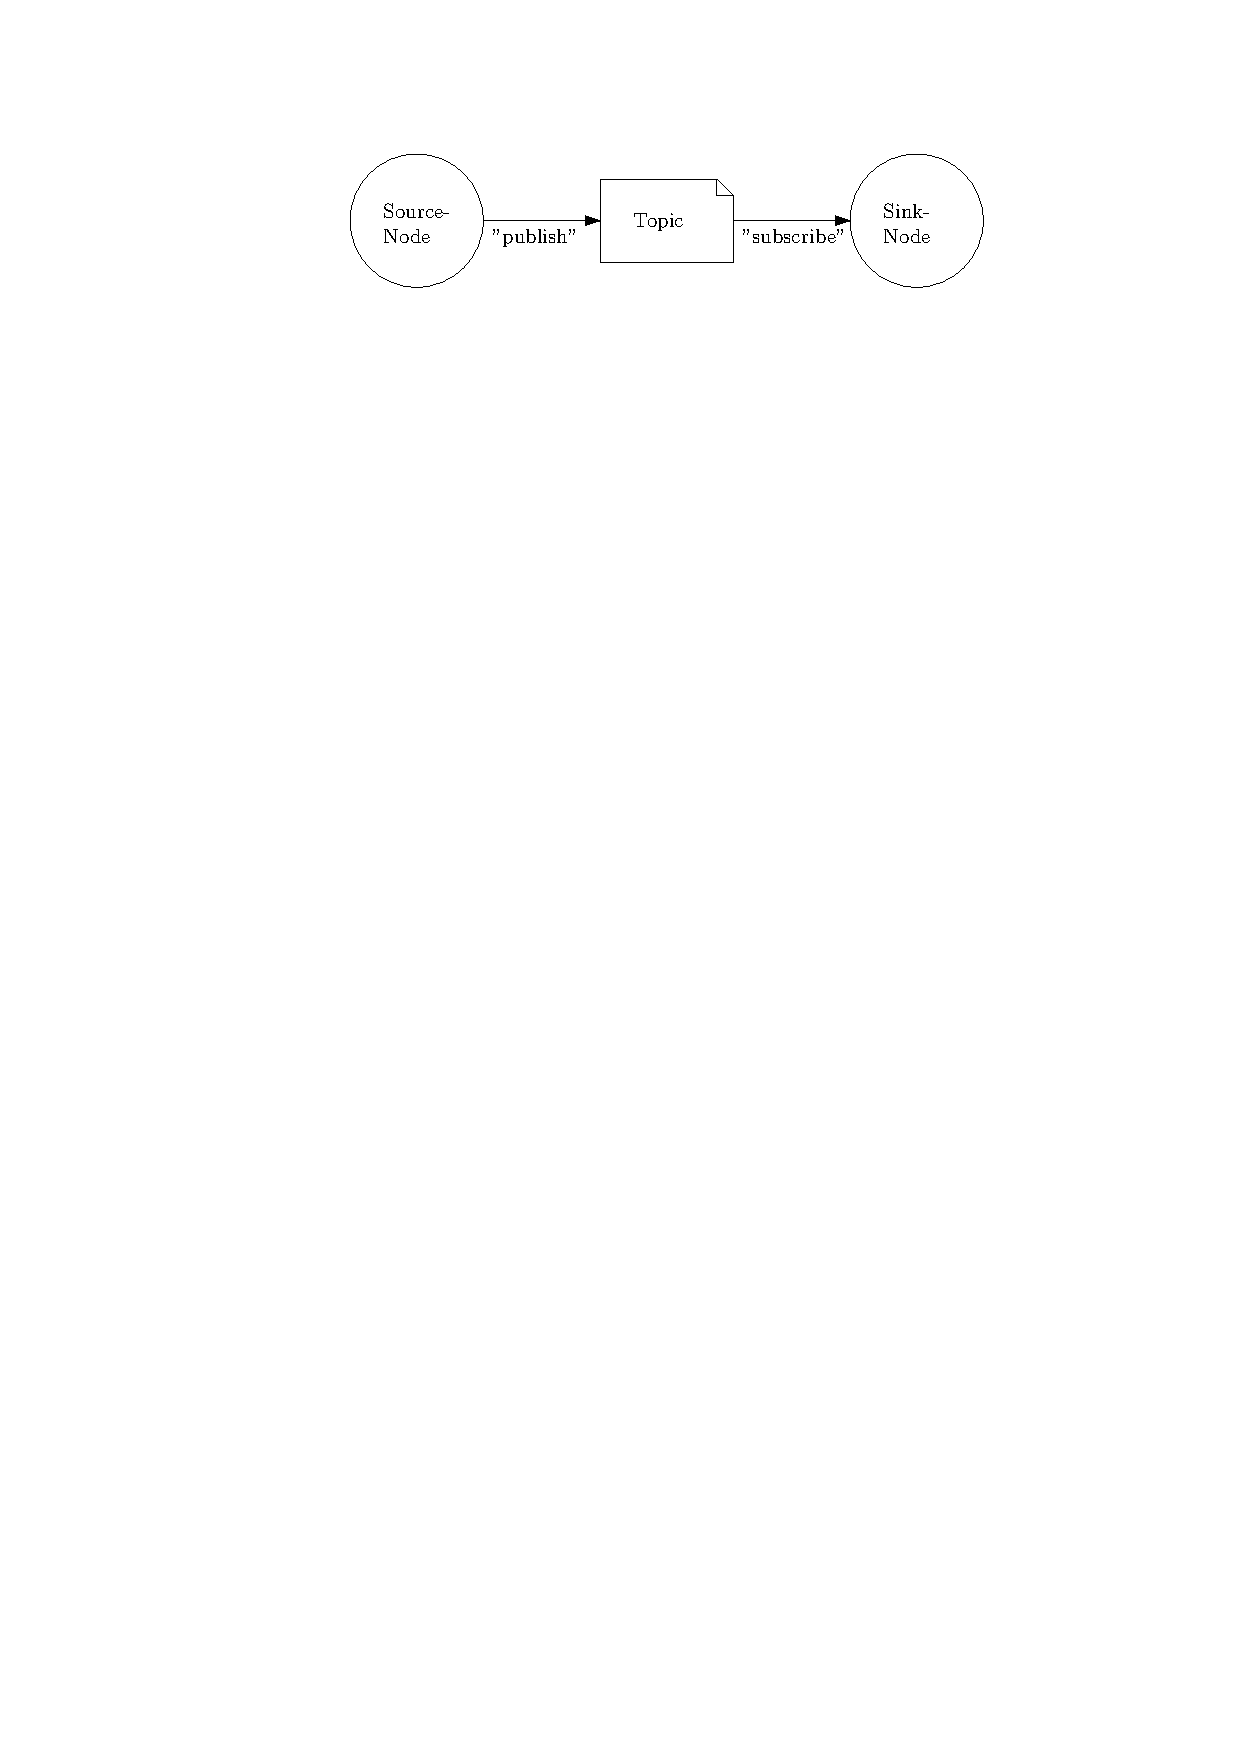
\includegraphics[width=0.6\textwidth]{ros-topic.pdf}
   \label{fig:ros_topic}
  \end{figure}
  \item \textbf{Unidirectional} communication
  \item \textit{Point to Point} and \textit{Point to Multipoint}
 \end{itemize}
\end{frame}
%----------------------------------------------------------------------------------------
\begin{frame}{Service}
 \begin{definition}[Service]
 \textit{Services allow for bidirectional communication between two nodes in form of request/response couples.}
 \end{definition}
 \begin{itemize}
  \item \textbf{Request} $\rightarrow$ $Node_1$ requests a service from $Node_2$ (e.g. addition)
  \item \textbf{Response} $\rightarrow$ $Node_2$ exetures service and returns result to $Node_2$
  \item 
   \begin{figure}[H]
    \centering
    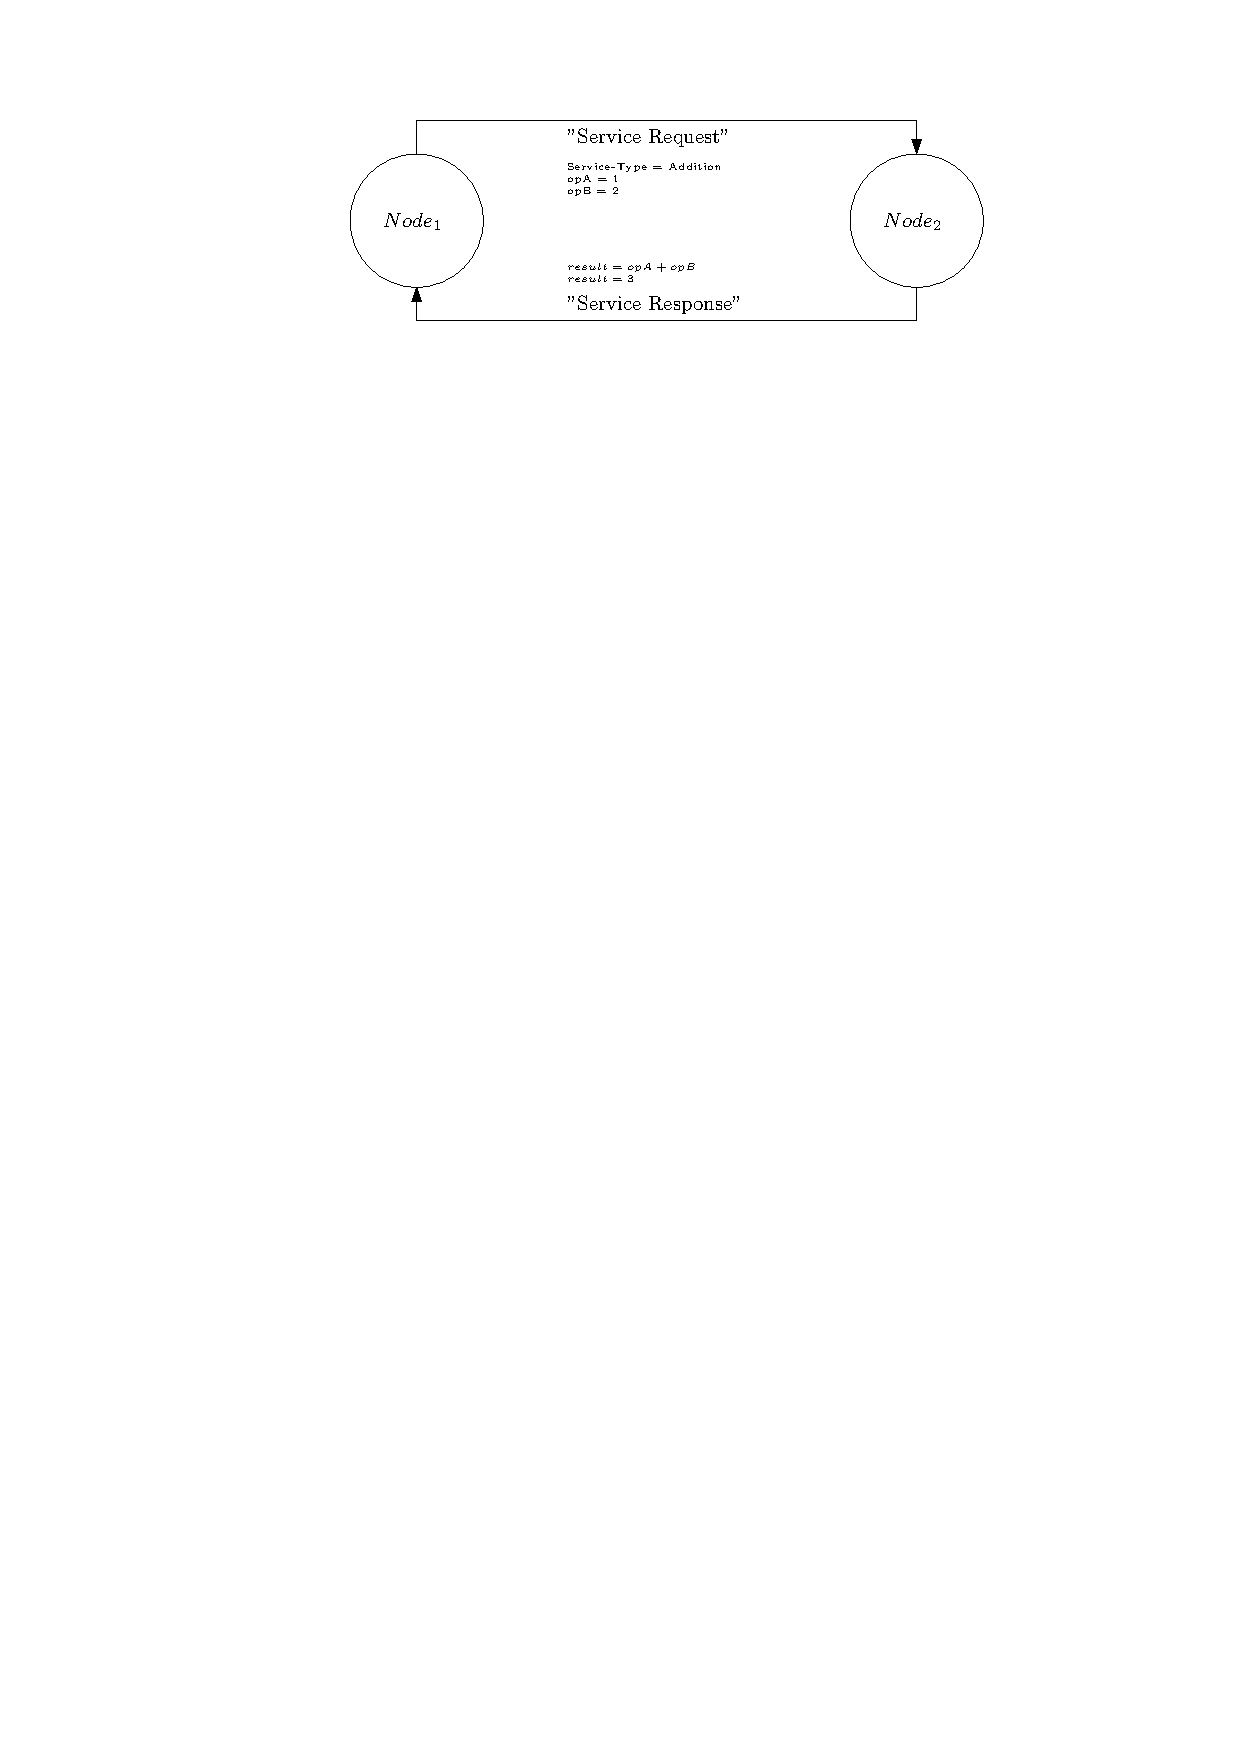
\includegraphics[width=0.6\textwidth]{ros-service.pdf}
    \label{fig:ros_service}
   \end{figure}
   \item Concrete implementation as a \textbf{remote procedure call}
   \item \textbf{Bidirectionale} (\textit{Point to Point}) communication
  \end{itemize}
\end{frame}
%----------------------------------------------------------------------------------------
\begin{frame}[allowframebreaks]{References}
\scriptsize{\bibliographystyle{ieeetr}}
\bibliography{references} %bibtex file name without .bib extension
\end{frame}
%----------------------------------------------------------------------------------------
\begin{frame}
\Huge{\centerline{The End}}
\end{frame}
%----------------------------------------------------------------------------------------
\end{document} 
%----------------------------------------------------------------------------------------